\documentclass[aspectratio=169, 11pt, invertlogo]{ismll-slides}
% - logo=[all, frametitle, headline, none]
% - logotitlepage=[true, false]
% - invertlogo: where to use white instead of black text (on transparent background)
% - nopdfpagenumbers: disable adding a number for each frame to pdf toc

%%%%%%%%%%%%%%%%
% BEAMER THEME %
%%%%%%%%%%%%%%%%
\usetheme[block=fill, background=light, progressbar=foot, numbering=counter]{metropolis}
%\usetheme{Madrid}
\setbeamertemplate{blocks}[default]
\setbeamercovered{transparent}

%%%%%%%%%%%%%%%%
% BIBLIOGRAPHY %
%%%%%%%%%%%%%%%%
% NOTE: Bibliography should be compiled with biber!
\addbibresource{slides-bibliography.bib}


%%%%%%%%%%%%%%%%%%%%%%%%%%
% TITLE PAGE INFORMATION %
%%%%%%%%%%%%%%%%%%%%%%%%%%

\title{Research Presentation}
\subtitle{Active Learning with V-Learning}
\author{Thorben Werner}
\date{March 31, 2022}
\institute{Information Systems and Machine Learning Lab (ISMLL)\\Institute for Computer Science \\ University of Hildesheim}



\begin{document}

%%%%%%%%%%%%%%%%%%%%%%%%%%%%%%%%%%%%%%%%%%%%%%%%%%%%%%%%%%%%%%%%%%%%%%%%%%%%%%%%%%%%%%%%%%%%%%%%%%%
\maketitle
%%%%%%%%%%%%%%%%%%%%%%%%%%%%%%%%%%%%%%%%%%%%%%%%%%%%%%%%%%%%%%%%%%%%%%%%%%%%%%%%%%%%%%%%%%%%%%%%%%%

\begin{frame}[fragile]{Pool-Based Active Learning}
	\begin{align*}
		\mathcal{L} &\in \mathbb{R}^{\lambda \times m} \hspace{3mm}\text{Labeled Set} \\
		\mathcal{U} &\in \mathbb{R}^{\mu \times m} \hspace{3mm}\text{Unlabeled Set} \\
		\phi_\theta &:= \mathbb{R}^{m} \rightarrow \mathbb{R}^{c} \hspace{3mm}\text{Classifier} \\
		\mathcal{K} &\in \mathbb{R}^{k \times m} \hspace{3mm}\text{Unlabeled Sample} \\
		\psi &:= \mathbb{R}^{k \times m} \rightarrow \mathbb{R}^k \hspace{3mm}\text{Active Learning Heuristic} \\
		\pi_\psi &:= argmax \hspace{1mm} \psi(\mathcal{S}) \hspace{3mm}\text{Active Learning Policy}
	\end{align*}
\end{frame}


%%%%%%%%%%%%%%%%%%%%%%%%%%%%%%%%%%%%%%%%%%%%%%%%%%%%%%%%%%%%%%%%%%%%%%%%%%%%%%%%%%%%%%%%%%%%%%%%%%%

\begin{frame}[fragile]{Active Learning with Q-Learning}
	\begin{columns}
		\begin{column}{.4\linewidth}
			\textbf{Problems:}
			\begin{itemize}
				\item Fixed Sample size
				\item Expensive Transitions
				\item Same actions in different places
			\end{itemize}
		\end{column}
		\begin{column}{.4\linewidth}
			\begin{align*}
				\mathcal{S} &\in \mathbb{R}^{b \times k \times \sigma} \hspace{3mm}\text{State Space} \\
				\mathcal{A} &\in [0, \ldots, k]^b \hspace{3mm}\text{Action Space} \\
				\mathcal{R} &:= \mathcal{S} \times \mathcal{A} \rightarrow \mathbb{R}^b \hspace{3mm}\text{Reward Function} \\
				\tau &:= \{ \mathcal{S}, \mathcal{A}, \mathcal{S}, \mathcal{R}, \mathbb{R}^b \} \hspace{3mm}\text{Transition} \\
			\end{align*}
		\end{column}
	\end{columns}
\end{frame}


%%%%%%%%%%%%%%%%%%%%%%%%%%%%%%%%%%%%%%%%%%%%%%%%%%%%%%%%%%%%%%%%%%%%%%%%%%%%%%%%%%%%%%%%%%%%%%%%%%%

\begin{frame}[fragile]{Active Learning with Q-Learning}
	\begin{columns}
		\begin{column}{.4\linewidth}
			\textbf{Sample siz}e $k = 2$ \\[2mm]
			The same datapoint can appear in multiple places in the input \\[2mm]
			Both output nodes essentially learn the same function
		\end{column}
		\begin{column}{.4\linewidth}
			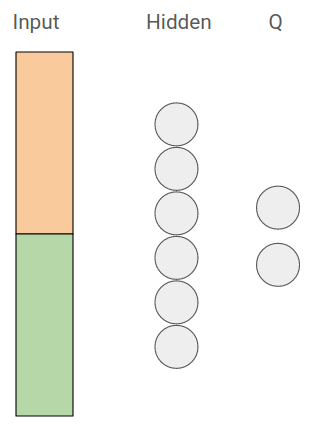
\includegraphics[width=120px]{pics/q}
		\end{column}
	\end{columns}
\end{frame}


%%%%%%%%%%%%%%%%%%%%%%%%%%%%%%%%%%%%%%%%%%%%%%%%%%%%%%%%%%%%%%%%%%%%%%%%%%%%%%%%%%%%%%%%%%%%%%%%%%%

\begin{frame}[fragile]{Active Learning with V-Learning}
	\begin{columns}
		\begin{column}{.4\linewidth}
			\textbf{Adaptations}
			\begin{itemize}
				\item We use the batch dimension for representing the sample size $k$
				\item No action space needed
				
			\end{itemize}
		\end{column}
		\begin{column}{.4\linewidth}
			\begin{align*}
			\mathcal{S} &\in \mathbb{R}^{b \times \sigma} \hspace{3mm}\text{State Space} \\
			\mathcal{R} &:= \mathcal{S} \rightarrow \mathbb{R} \hspace{3mm}\text{Reward Function} \\
			\end{align*}
		\end{column}
	\end{columns}
\end{frame}


%%%%%%%%%%%%%%%%%%%%%%%%%%%%%%%%%%%%%%%%%%%%%%%%%%%%%%%%%%%%%%%%%%%%%%%%%%%%%%%%%%%%%%%%%%%%%%%%%%%

\begin{frame}[fragile]{Storing Transitions in Memory}
	Q-Learning:
	\begin{align*}
		O(\tau) &= \mathcal{S} \times \mathcal{A} \times \mathcal{S} \times \mathcal{R} \times \mathbb{R} \\
		O(\tau) &= k^2 \times \sigma^2 + 3
	\end{align*}
	V-Learning:
	\begin{align*}
		O(\tau) &= \mathcal{S} \times \mathcal{A} \times \mathcal{S} \times \mathcal{R} \times \mathbb{R} \\
		O(\tau) &= 2 \times \sigma^2 + 3
	\end{align*}
\end{frame}



%%%%%%%%%%%%%%%%%%%%%%%%%%%%%%%%%%%%%%%%%%%%%%%%%%%%%%%%%%%%%%%%%%%%%%%%%%%%%%%%%%%%%%%%%%%%%%%%%%%

\begin{frame}[fragile]{Pool-Based Active Learning}
	some
\end{frame}



%%%%%%%%%%%%%%%%%%%%%%%%%%%%%%%%%%%%%%%%%%%%%%%%%%%%%%%%%%%%%%%%%%%%%%%%%%%%%%%%%%%%%%%%%%%%%%%%%%%
\appendix
%%%%%%%%%%%%%%%%%%%%%%%%%%%%%%%%%%%%%%%%%%%%%%%%%%%%%%%%%%%%%%%%%%%%%%%%%%%%%%%%%%%%%%%%%%%%%%%%%%%


%\begin{frame}[fragile]{Backup Slides}
%
%\begin{block}<1->{Did you know?}%
%  Pages after the \verb|\appendix| command do not get counted in the page total.
%\end{block}%
%
%\end{frame}


%%%%%%%%%%%%%%%%%%%%%%%%%%%%%%%%%%%%%%%%%%%%%%%%%%%%%%%%%%%%%%%%%%%%%%%%%%%%%%%%%%%%%%%%%%%%%%%%%%%


\begin{frame}[allowframebreaks]%{References}
%
%\printbibliography%[heading=none]
%
\end{frame}

%%%%%%%%%%%%%%%%%%%%%%%%%%%%%%%%%%%%%%%%%%%%%%%%%%%%%%%%%%%%%%%%%%%%%%%%%%%%%%%%%%%%%%%%%%%%%%%%%%%


\end{document}
